%!TEX options = --shell-escape

\documentclass[bachelor]{thesis-uestc}

\title{UESTC Thesis Template}
\author{张义飞}

\begin{document}
	
	\begin{chineseabstract}
		[TODO]
		
		\chinesekeyword{强化学习,虚拟现实,机器控制算法}
	\end{chineseabstract}
	
	\begin{englishabstract}
		[TODO]
		\englishkeyword{Reinforcement Learning, Virtual Reality, Robotic Control}
	\end{englishabstract}
	
	\thesistableofcontents
	
	\thesischapterexordium
	
	\section{研究工作的背景与意义}
	
	机器学习是以知识的自动获取和产生为研究目标,是人工智能的核心问题之一。机器学习与统计学、心理学、机器人学等许多其他学科都有交叉。其中,学习心理学与机器学习的交叉综合直接促进了强化学习又称做增强学习或再励学习(Reinforcement Learning,RL) 理论与算法的产生和发展。所谓强化学习是一种以环境反馈作为输入的、特殊的、适应环境的机器学习方法,它的主要思想是与环境交互和试错,利用评价性的反馈信号实现决策的优化。这也是自然界中人类或动物学习的基本途径。
	
	近年来,强化学习技术在人工智能、机器学习和自动控制等领域中得到了广泛的研究和应用,并被认为是设计智能系统的核心技术之一。随着强化学习算法和理论的深入,特别是强化学习的数学基础研究取得突破性进展之后,应用强化学习方法实现移动机器人行为对环境的自适应和控制器的优化成为机器人学领域研究和应用的热点之一。
	
	与此同时,虚拟现实技术已被认为是人机接口技术的一场革命。它利用计算机和电子技术来产生逼真的视、听、触、力等三维感觉环境, 形成一种虚拟世界。 它与人工智能、计算机图形学、人机接口技术、多媒体技术、传感技术以及高度并行的实时计算技术等领域联系十分紧密。虚拟现实技术可以最大限度地模拟真实环境,根据这个特点,人们可以在虚拟现实中开展各种训练任务,训练完成后将模型迁移到真实环境中。
	
	\section{强化学习算法的国内外研究历史与现状}
	强化学习作为机器学习领域另一个研究热点,已经广泛应用于工业制造。因此RL 方法更加侧重于学习解决问题的策略。随着人类社会的飞速发展,在越来越多复杂的现实场景任务中,需要利用深度学习(Deep Learning, DL)来自动学习大规模输入数据的抽象表征,并以此表征为依据进行自我激励的RL,优化解决问题的策略。RL的基本思想是通过最大化智能体(agent)从环境中获得的累计奖赏值,以学习到完成目标的最优策略。由此,谷歌的人工智能研究团队DeepMind 创新性地将具有感知能力的DL和具有决策能力的RL相结合,形成了人工智能领域新的研究热点,即深度强化学习(Deep Reinforcement Learning,DRL)。此后,在很多挑战性领域中,DeepMind 团队构造并实现了人类专家级别的agent。这些agent 对自身知识的构建和学习都直接来自原始输入信号,无需任何的人工编码和领域知识。因此DRL 是一种端对端(end-to-end)的感知与控制系统,具有很强的通用性。目前DRL技术在游戏等领域中得到了广泛的应用,并被认为是迈向通用人工智能(Artificial General Intelligence,AGI)的重要途径。
	
	\begin{figure}
		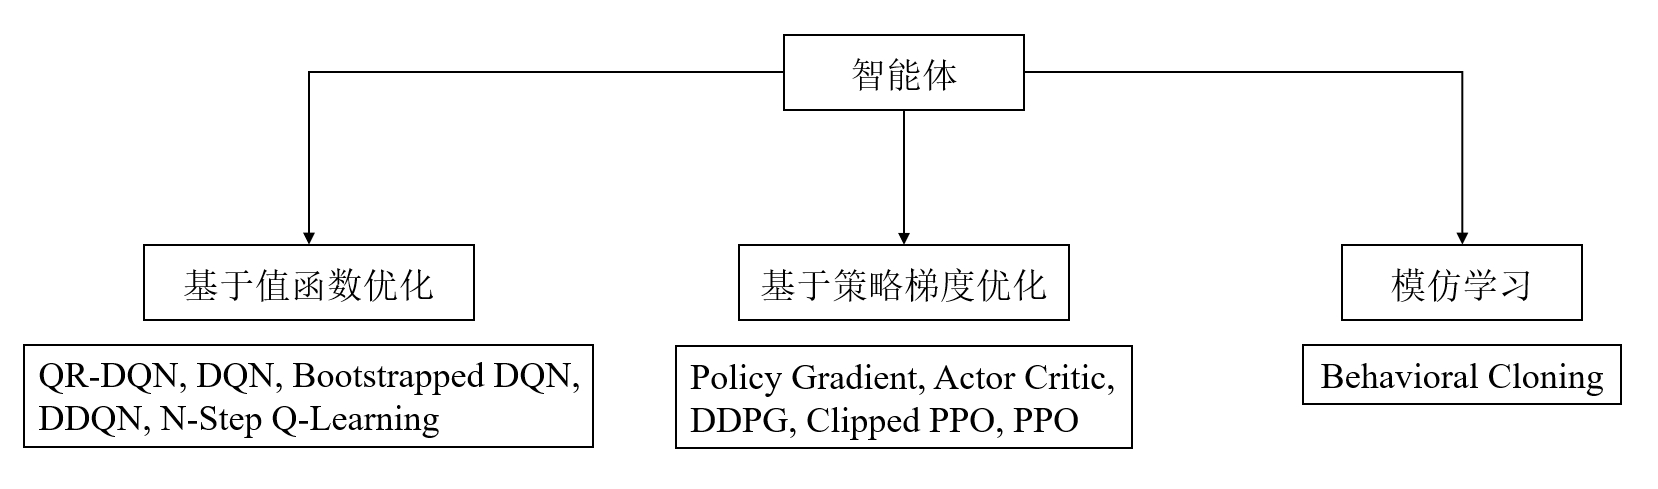
\includegraphics[width=15cm]{./pic/fg6.jpg}
		\caption{主流强化学习算法}
		\label{fg6}
	\end{figure}
	
	如图\ref{fg6}所示,目前主流的强化学习算法主要分为如下几类:
	\begin{enumerate}
		\item 基于值函数优化(Value Optimization)的算法,代表算法为Q-Learning,Mnih 等人将卷积神经网络与传统RL中的Q-Learning算法相结合,提出了深度Q网络(Deep Q-Network, DQN)模型,此后又涌现出双深度Q网络(Double Deep Q-Network, DDQN)、分类Q网络(Categorical Deep Q-Network,CDQN)、增强Q网络(Bootstrapped Deep Q-Network)等一系列值优化模型;
		
		\item 基于策略梯度优化(Policy Optimization)的算法,此类算法可以能够直接在策略空间中搜索最优策略,从而比基于值函数优化的方法实用性更广,代表算法有区域信赖的策略最优化方法(Trust Region Policy Optimization,TRPO)、近端梯度优化方法(Proximal Policy Optimization, PPO)。
		
		\item 行动者-评论者优化方法(Actor-Critic),Lillicrap 等人利用DQN扩展Q-Learning的思路对确定性梯度策略(Deterministic Policy Gradient,DPG)方法进行改造,提出了一种基于AC 框架的深度确定性策略梯度(Deep Deterministic Policy Gradient,DDPG)算法,并在解决连续动作空间问题上取得了很好的效果。
	\end{enumerate}
	
	\section{本文的主要贡献与创新}
	本文尝试将Unity 3D环境与强化学习算法的训练过程结合起来,使得强化学习的训练时间大幅度减少。并且通过Unity强大的物理引擎尽可能地拟合真实环境,从而使得训练出的强化学习模型无需经过细致调参优化就可以很好地迁移应用到实体机械环境上。
	
	\section{本论文的结构安排}
	本文的主要章节安排如下:第二章主要介绍了强化学习领域的基础知识,并对主流的强化学习算法进行对比介绍;第三章则介绍目前强化学习在机器控制领域的主流仿真环境,并将其与Unity进行对比;第四章介绍架构的组成。
	
	\chapter{强化学习理论}
	\section{强化学习基础}
	RL是一种从环境状态映射到动作的学习,目标是使agent在与环境的交互过程中获得最大的累积奖赏。马尔可夫决策过程(Markov Decision Process,MDP)可以用来对RL问题进行建模。通常将MDP 定义为一个四元组$(S,A,\rho,f)$,其中:
	
	\begin{enumerate}
		\item $S$为所有环境状态的集合。$s_t\in S$表示agent在$t$时刻所处的状态;
		\item $A$为agent可执行动作的集合。$a_t\in A$表示agent在$t$时刻所采取的动作;
		\item $\rho:S\times A\rightarrow R$为奖赏函数。$r_t\sim \rho(s_t,a_t)$表示agent在状态执行动作获得的立即奖赏值;
		\item $f:S\times A\times S\rightarrow [0,1]$为状态转移概率分布函数。$S_{t+1}\sim f(s_t,a_t)$表示agent在状态$s_t$执行动作$a_t$转移到下一状态$S_{t+1}$的概率。
	\end{enumerate}
	
	在RL中,策略$\pi :S\rightarrow A$是状态空间到动作空间的一个映射。表示为agent在状态$s_t$选择动作$a_t$,执行该动作并以概率$f(s_t,a_t)$转移到下一状态$s_{t+1}$,同时接受来自环境反馈地奖赏$r_t$。假设未来每个时间步所获得的立即奖赏都必须乘以一个折扣因子$\gamma$,则从$t$时刻开始到$T$时刻结束时,奖赏之和定义为:
	\begin{equation}\label{eq1}
	R_t=\sum^T_{t'=t}\gamma^{t'-t}r_t
	\end{equation}
	
	其中$\gamma\in [0,1]$,用来权衡未来奖赏对累计奖赏的影响。
	状态动作值函数$Q^\pi (s,a)$指的是在当前状态$s$下执行该动作$a$,并一直遵循策略$\pi$到情节结束,这一过程中agent所获得的累计回报表示为:
	\begin{equation}\label{eq2}
	Q^\pi (s,a)=E[R_t|s_t=s,a_t=a,\pi]
	\end{equation}
	
	对于所有的状态动作对,如果一个策略$\pi ^*$的期望回报大于或等于其他所有策略的期望回报,那么称策略$\pi ^*$为最优策略。最优策略可能不只一个,但它们共享一个状态动作值函数:
	\begin{equation}\label{eq3}
	Q^\pi (s,a)=max_\pi E[R_t|s_t=s,a_t=a,\pi]
	\end{equation}
	
	式\ref{eq3}被称为最优状态值函数,且最优状态动作值函数遵循贝尔曼最优方程(Bellman Optimality Equation)。即:
	\begin{equation}
	\label{eq4}
	Q^*(s,a)=E_{s'\sim S}[r+\gamma max_{a'}Q(s',a')|s,a]
	\end{equation}
	
	在传统的RL中,一般通过迭代贝尔曼方程求解Q值函数:
	\begin{equation}
	\label{eq5}
	Q_{i+1}(s,a)=E_{s'\sim S}[r+\gamma max_{a'}Q_i(s',a')|s,a]
	\end{equation}
	
	其中,当$i\rightarrow\infty$时,$Q_i\rightarrow Q^*$。即通过不断地迭代会使状态动作值函数最终收敛,从而得到最优策略$\pi^*=argmax_{a\in A}Q^*(s,a)$。然而对于实际问题来说,通过迭代式\ref{eq5}求解最优策略显然是不可行的,因为在大状态空间下,用迭代贝尔曼方程求解$Q$值函数的方法计算代价太大.针对此问题,在RL算法中,通常使用线性函数逼近器来近似表示状态动作值函数,即$Q(s,a,\theta)\approx Q^*(s,a)$。此外,也可以用深度神经网络等非线性函数逼近器去近似表示值函数或策略。然而将RL与深度神经网络相结合可能会出现算法不稳定等问题,这一直阻碍着DRL的发展与应用。
	
	\section{基于值函数的深度强化学习}
	\subsection{深度Q网络}
	Mnih等人将卷积神经网络与传统RL中的Q学习算法相结合,提出了深度Q网络(Deep Q-Network, DQN)模型.该模型用于处理基于视觉感知的控制任务,是DRL领域的开创性工作.
	
	\subsubsection{模型结构}
	DQN模型的输入是距离当前时刻最近的4幅预处理后的图像。该输入经过3个卷积层和2个全连接层的非线性变换,最终在输出层产生每个动作的Q值。图\ref{fg1}表示DQN的模型结构。
	\begin{figure}
		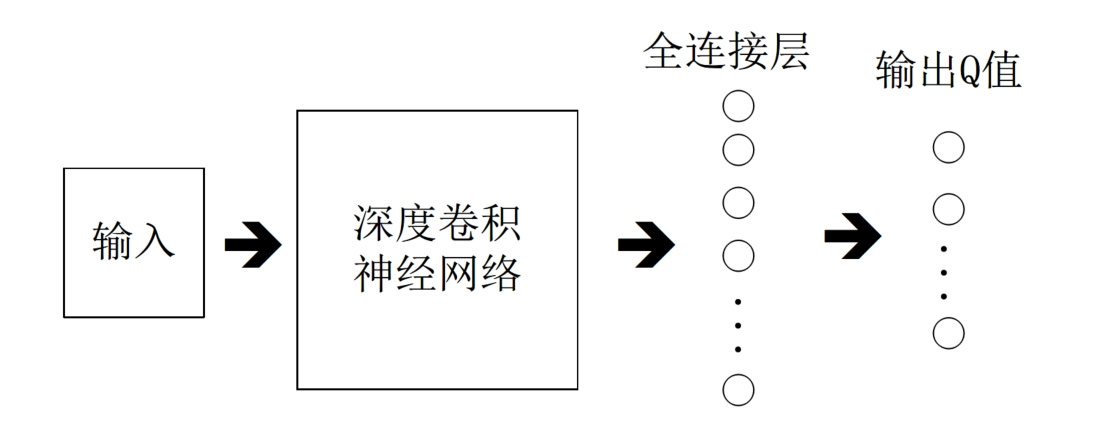
\includegraphics[width=8cm]{./pic/fg1.jpg}
		\caption{DQN的模型结构}
		\label{fg1}
	\end{figure}
	
	\subsubsection{训练算法}
	\begin{figure}
		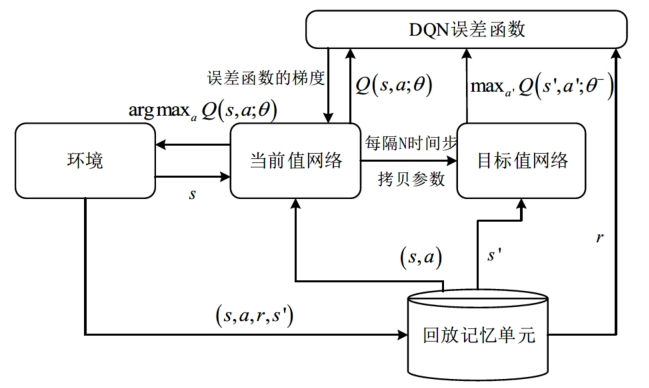
\includegraphics[width=10cm]{./pic/fg2.jpg}
		\caption{DQN的训练过程}
		\label{fg2}
	\end{figure}
	图\ref{fg2}描述了DQN的训练过程。为缓解非线性网络表示值函数时出现的不稳定等问题,DQN主要对传统的Q学习算法做了3处改进。
	
	\begin{enumerate}
		\item DQN在训练过程中使用经验回放机制(experience replay),在线处理得到的转移样本$e_t=(s_t,a_t,r_t,s_{t+1})$。在每个时间步$t$,将agent与环境交互得到的转移样本存储到回放记忆单元$D={e_1,...e_t}$中。训练时,每次从$D$中随机抽取小批量的转移样本,并使用随机梯度下降(Stochastic Gradient Descent, SGD)算法更新网络参数$\theta$。在训练深度网络时,通常要求样本之间是相互独立的。这种随机采样的方式,大大降低了样本之间的关联性,从而提升了算法的稳定性。
		
		\item DQN除了使用深度卷积网络近似表示当前的值函数之外,还单独使用了另一个网络产生目标Q值。具体地,$Q(s,a|\theta_i)$表示当前值网络的输出,用来评估当前状态动作对的值函数;$Q(s,a|\theta^-_i)$表示目标值网络的输出,一般采用近似表示值函数的优化目标,即目标Q值.当前值网络的参数$\theta$是实时更新的,每经过N轮迭代,将当前值网络的参数复制给目标值网络。通过最小化当前Q值和目标Q值之间的均方误差来更新网络参数,误差函数为:
		\begin{equation}
			\label{eq6}
			L(\theta_i)=E_{s,a,r,s'}[(Y_i-Q(s,a|\theta_i))^2]
		\end{equation}
		对参数$\theta$求偏导,得到一下梯度:
		\begin{equation}
			\label{eq7}
			\nabla_{\theta_i}=E_{s,a,r,s'}[(Y_i-Q(s,a|\theta_i))\nabla_{\theta_i}Q(s,a|\theta_i)]
		\end{equation}
		引入目标值网络后,在一段时间内目标Q值是保持不变的,一定程度上降低了当前Q值和目标Q值之间的相关性,提升了算法的稳定性。
		
		\item DQN将奖赏值和误差项缩小到有限的区间内,保证了Q值和梯度值都处于合理的范围内,提高了算法的稳定性。实验表明,DQN在解决诸如Atari 2600游戏等类真实环境的复杂问题时,表现出与人类玩家相媲美的竞技水平,甚至在一些难度较低的非战略性游戏中,DQN的表现超过了有经验的人类玩家。在解决各类基于视觉感知的DRL任务时,DQN使用了同一套网络模型、参数设置和训练算法,这充分说明DQN方法具有很强的适应性和通用性。
	\end{enumerate}

	\subsection{深度Q网络训练算法的改进}
	\subsubsection{深度双Q网络}\label{sec1}
	在DQN中使用$Y_i=r+\gamma max_{a'}Q(s',a'|\theta_i^-)$近似表示值函数的优化目标时,每次都选取下一个状态中最大Q值所对应的动作。选择和评价动作都是基于目标值网络的参数$\theta^-$,这会引起在学习过程中出现过高估计Q值的问题。
	
	Hasselt等人基于双Q学习算法(double Q-learning),提出了深度双Q网络(Deep DoubleQ-Network, DDQN)算法。在双Q学习中有两套不同的参数:$\theta$和$\theta^-$。其中$\theta$用来选择对应最大Q值的动作,$\theta$用来评估最优动作的Q值。两套参数将动作选择和策略评估分离开,降低了过高估计Q值的风险。因此DDQN使用当前值网络的参数$\theta$来选择最优动作,使用目标值网络的参数$\theta^-$来评估该最优动作。目标Q值的形式如下:
	\begin{equation}
		\label{eq8}
		Y_i^{DDQN}=r+\gamma Q(x',argmax_a Q(s',a'|\theta_i^-))
	\end{equation}
	DDQN在其他方面都与DQN保持一致。实验表明,DDQN能够估计出更加准确的Q值,在一些Atari 2600游戏中可获得更稳定有效的策略。
	
	\subsubsection{基于优势学习的深度Q网络}
	根据\ref{sec1}节可知,降低Q值的评估误差可以提升性能。Bellemare等人在贝尔曼方程中定义新的操作符,来增大最优动作值和次优动作值之间的差异,以缓和每次都选取下一状态中最大Q值对应动作所带来的评估误差。具体的改进如下:
	基于采样得到的样本计算均方误差$\Delta Q(s,a)^2$,其中误差项定义为:
	\begin{equation}
		\label{eq9}
		\Delta Q(s,a)=r+\gamma V(s')-Q(s,a)
	\end{equation}
	根据优势学习(Advantage Learning,AL)定义两种新的操作符,并将这两种操作符运用到上式中,分别得到AL误差项和一致性优势学习(Persistent Advantage Learning,PAL)误差项。其中AL误差项定义为:
	\begin{equation}
		\label{eq10}
		\Delta_{AL}Q(s,a)=\Delta Q(s,a)-\alpha[V(s)-Q(s,a)]
	\end{equation}
	为了定义PAL误差项,构造出如下式:
	\begin{equation}
		\label{eq11}
		\Delta_{AL}Q'(s,a)=\Delta Q(s',a)-\alpha[V(s)-Q(s',a)]
	\end{equation}
	得到PAL误差项的具体形式:
	\begin{equation}
		\label{eq12}
		\Delta_{PAL}Q(s,a)=max{\Delta_{AL}Q(s,a),\Delta_{AL}Q'(s,a)}
	\end{equation}
	实验表明,用AL和PAL误差项来替代贝尔曼方程中的误差项,可以有效地增加最优和次优动作对应值函数之间的差异,从而获得更加精确的Q值。即在DQN中加入AL和PAL误差项,可以有效地减小评估Q值时的偏差,促进学习效果的进一步提升,在许多Atari 2600游戏中取得了更好的表现。其中,采用PAL误差项时,最优和次优动作对应值函数之间的差异更大,Q值的评估也更加精确。
	
	\subsubsection{基于优先级采样的深度Q网络}
	DQN为了消除转移样本$e_t=(s_t,a_t,r_t,s_{t+1})$之间的相关性,使用经验回放机制在线地存储和使用agent与环境交互得到的历史样本。在每个时刻,经验回放机制从样本池中等概率地抽取小批量的样本用于训练。然而等概率采样并不能区分不同样本的重要性,同时由于样本池D的存储量有限,某些样本还未被充分利用就已经被舍弃。针对该问题,Schaul等人在DDQN的基础上提出了一种基于比例优先级采样的深度双Q网络(double deep Q-Network with proportional prioritization)。该方法用基于优先级的采样方式来替代均匀采样,提高一些有价值样本的采样概率,从而加快最优策略的学习。具体的改进如下:

	该抽样方法将每个样本的时间差分(Temporal Difference,TD)误差项作为评价优先级的标准。该误差为:$r+\gamma max_{a'}Q(s',a'|\theta^-)-Q(s,a|\theta)$,并且其绝对值越大,对应样本被采样的概率越高。在抽样过程中该方法使用随机比例化(stochastic prioritization)和重要性采样权重(importance-sampling weights)两种技巧。其中,随机比例化操作不仅能充分利用较大TD误差项对应的样本,而且保证了抽取样本的多样性。重要性采样权重的使用放缓了参数更新的速度,保证了学习的稳定性。实验表明,基于该抽样方式的深度双Q网络可以提升训练速度,并在很多Atari 2600游戏中获得了更高的分数。
	
	另外,Lakshminarayanan等人使用动态跳帧的方式来替代DQN中每个时刻重复k次的动作,提出了动态跳帧的DQN(Dynamic Frame Skip DeepQ-Network,DFDQN)算法。实验表明,DFDQN在一些Atari 2600游戏中取得了更好的性能;Hasselt等人使用一种称为Pop-Art的动态归一化操作来替代传统DQN中的区间裁剪方法。在不流失重要状态信息的前提下,统一了不同任务中目标Q值的量级,提高了agent在很多Atari2600游戏中的表现;Vincent等人在DQN中使用自适应的折扣因子和学习率,加速了深度网络收敛的速度。
	
	\subsection{DQN模型结构的改进}
	对DQN模型的改进一般是通过向原有网络中添加新的功能模块来实现的。例如,可以向DQN模型中加入循环神经网络结构,使得模型拥有时间轴上的记忆能力。本节主要介绍两种重要的DQN模型的改进版本,分别是基于竞争架构的DQN和深度循环Q网络(Deep Recurrent Q-Network,DRQN)。
	\subsubsection{基于竞争架构的DQN}
	在很多基于视觉感知的DRL任务中,受不同动作的影响,状态动作对的值函数是不同的。然而在某些状态下,值函数的大小是与动作无关的。利用上述思想,Wang等人设计了一种竞争网络结构(dueling network),并将其加入到DQN网络模型中。如图\ref{fg3},该网络结构与DQN模型的不同之处在于:DQN将CNN提取的抽象特征经过全连接层后,直接在输出层输出对应动作的Q值,而引入竞争网络结构的模型则将CNN提取的抽象特征分流到两个支路中,其中一路代表状态值函数,另一路代表依赖状态的动作优势函数(advantage function)。通过该种竞争网络结构,agent可以在策略评估过程中更快地识别出正确的行为。
	\begin{figure}
		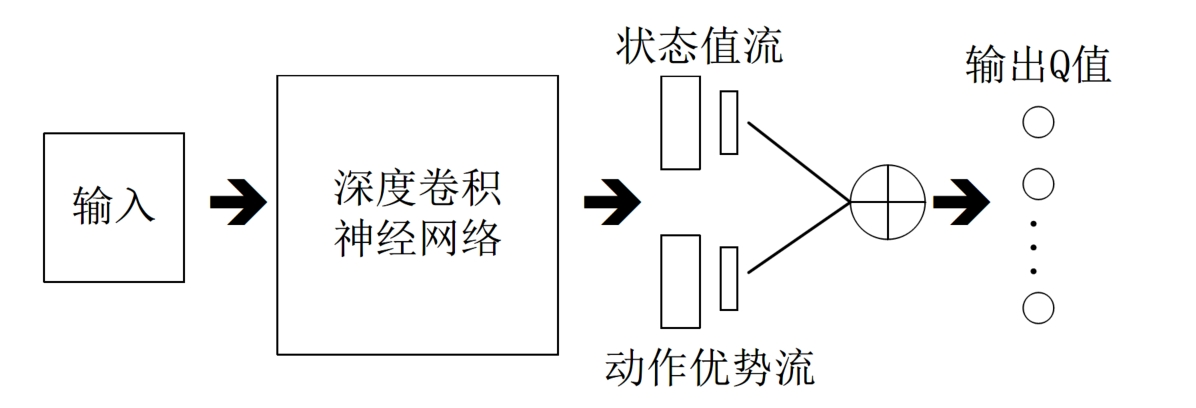
\includegraphics[width=8cm]{./pic/fg3.jpg}
		\caption{基于竞争架构的DQN模型结构}
		\label{fg3}
	\end{figure}
	具体地,状态值函数表示为$\hat{V}(s|\theta,\beta)$,动作优势函数表示为$\hat{A}(s,a|\theta,\alpha)$。通过一种聚合操作将状态值流和动作优势流相结合:
	\begin{equation}
		\label{eq13}
		Q(s,a|\theta,\alpha,\beta)=\hat{V}(s|\theta,\beta)+\hat{A}(s,a|\theta,\alpha)
	\end{equation}
	其中,$\alpha$、$\beta$和$\theta$分别代表状态值流、动作优势流和模型剩余部件的参数。然而在实际操作中,一般要将动作优势流设置为单独动作优势函数值减去某状态下所有动作优势函数的平均值。该技巧不仅可以保证该状态下各动作的优势函数相对排序不变,而且可以缩小Q值的范围,去除多余的自由度。实验表明,在DQN中加入竞争网络可以使得值函数的估计更加精确。在频繁出现agent采取不同动作但对应值函数相等的情形下,竞争架构的DQN模型性能提升最为明显。
	
	\subsubsection{深度循环Q网络}
	在传统的RL方法中,状态信息的部分可观察性一直是个亟待解决的难题。DQN通过堆叠离当前时刻最近的4幅历史图像组成输入状态,有效缓解了状态信息的部分可观察问题,却增加了网络的计算和存储负担。针对此问题,Hausknecht等人利用循环神经网络结构来记忆时间轴上连续的历史状态信息,提出了DRQN模型。
	\begin{figure}
		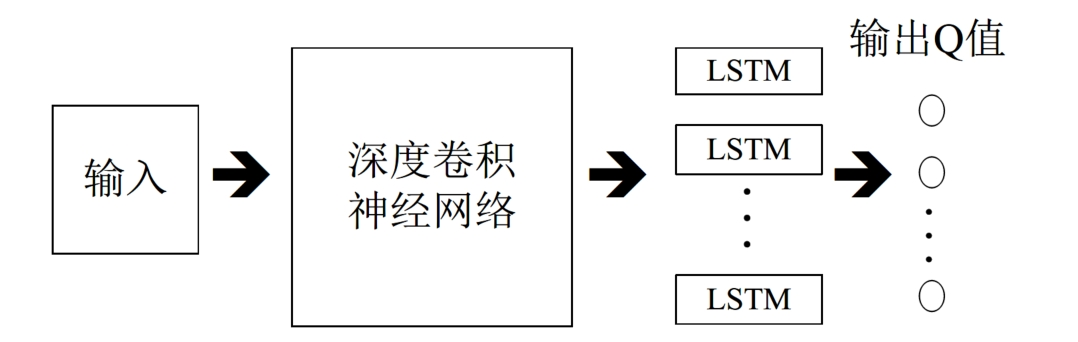
\includegraphics[width=8cm]{./pic/fg4.jpg}
		\caption{DRQN模型结构}
		\label{fg4}
	\end{figure}
	如图\ref{fg4}所示,DRQN将DQN中第1个全连接层的部件替换成了256个长短期记忆单元(Long Short-TermMemory,LSTM)。此时模型的输入仅为当前时刻的一幅图像,减少了深度网络感知图像特征所耗费的计算资源。实验表明,在部分状态可观察的情况下,DRQN表现出比DQN更好的性能。因此DRQN模型适用于普遍存在部分状态可观察问题的复杂任务。
	
	随着DL领域中各种新颖网络模块的提出,未来DRL模型会朝着结构多样化、模块复杂化的方向发展。例如,可以利用深度残差网络所具备的强大感知能力来提高agent对复杂状态空间的表征效果;另外,可以在模型中加入视觉注意力机制(Visual Attention Mechanism,VAM),使得agent在不同状态下将注意力集中到有利于做出决策的区域,从而加速学习的进程。
	
	\section{基于策略梯度的深度强化学习}
	策略梯度是一种常用的策略优化方法,它通过不断计算策略期望总奖赏关于策略参数的梯度来更新策略参数,最终收敛于最优策略。因此在解决DRL问题时,可以采用参数为的深度神经网络来进行参数化表示策略,并利用策略梯度方法来优化策略。值得注意的是,在求解DRL问题时,往往第一选择是采取基于策略梯度的算法。原因是它能够直接优化策略的期望总奖赏,并以端对端的方式直接在策略空间中搜索最优策略,省去了繁琐的中间环节。因此与DQN及其改进模型相比,基于策略梯度的DRL方法适用范围更广,策略优化的效果也更好。
	\subsection{深度策略梯度的起源与发展}\label{sec2}
	策略梯度方法是一种直接使用逼近器来近似表示和优化策略,最终得到最优策略的方法。该方法优化的是策略的期望总奖赏:
	\begin{equation}
		\label{eq14}
		max_{\theta}E[R|\pi_\theta]
	\end{equation}
	其中$R=\sum_{t=0}^{T-1}$表示一个情节内所获得的奖赏总和。策略梯度最常见的思想是增加总奖赏较高情节出现的概率。策略梯度方法的具体过程如下:
	假设一个完整情节的状态、动作和奖赏的轨迹为:$\tau=(s_0,a_0,r_0,s_1,a_1,r_1,...,s_{T-1},a_{T-1},r_{T-1},s_T)$。则策略梯度表示为如下的形式:
	\begin{equation}
		\label{eq15}
		g=R\nabla_\theta\sum_{t=0}^{T-1}log\pi(a_t|s_t;\theta)
	\end{equation}
	利用该梯度调整策略参数:
	\begin{equation}
		\label{eq16}
		\theta\leftarrow\theta+\alpha g
	\end{equation}
	其中,$\alpha$是学习率,控制着策略参数更新的速率。式\ref{eq15}中的$\nabla_\theta\sum_{t=0}^{T-1}log\pi(a_t|s_t;\theta)$梯度项表示能够提高轨迹$\tau$出现概率的方向,乘以得分函数R之后,可以使得单个情节内总奖赏越高的$\tau$概率密度越大。即如果收集了很多总奖赏不同的轨迹,通过上述训练过程会使得概率密度向总奖赏更高的轨迹方向移动,最大化高奖赏轨迹$\tau$出现的概率。
	然而在某些情形下,每个情节的总奖赏R都不为负,那么所有梯度g的值也都是大于等于0的。此时在训练过程中遇到每个轨迹$\tau$,都会使概率密度向正的方向“拉拢”,很大程度减缓了学习速度。这会使得梯度g的方差很大。因此可以对R使用某种标准化操作来降低梯度g的方差。该技巧使得算法能提高总奖赏R较大的轨迹$\tau$的出现概率,同时降低总奖赏R较小的轨迹$\tau$出现概率。根据上述思想,Williams等人提出了REINFORCE算法,将策略梯度的形式统一为:
	\begin{equation}
		\label{eq17}
		g=\nabla_\theta\sum_{t=0}^{T-1}log\pi(a_t|s_t;\theta)(R-b)
	\end{equation}
	其中,b是一个与当前轨迹$\tau$相关的基线,通常设置为R的一个期望估计,目的是减小R的方差。可以看出,R超过基准b越多,对应的轨迹$\tau$被选中的概率越大。因此在大规模状态的DRL任务中,可以通过深度神经网络参数化表示策略,并采用传统的策略梯度方法来求解最优策略。
	
	此外,优化策略的另一种思路是增加“好”的动作出现的概率。在RL中一般是通过优势函数评价动作的好坏,因此可以利用优势函数项来构造策略梯度:
	\begin{equation}
		\label{eq18}
		g=\nabla_\theta\sum_{t=0}^{T-1}\hat{A}log\pi(a_t|s_t;\theta)
	\end{equation}
	其中$\hat{A_t}$表示状态动作对$(s_t,a_t)$优势函数的一个估计,通常构造成以下形式:
	\begin{equation}
		\label{eq19}
		\hat{A_t^\gamma}=r_t+\gamma r_{t+1}+\gamma^2 r_{t+2}+\dots-V(s_t)
	\end{equation}
	其中,$\gamma\in[0,1]$表示折扣因子。此时带折扣的奖赏之和$r_t+\gamma r_{t+1}+\gamma^2 r_{t+2}+\dots$相当于式\ref{eq17}中的R,带折扣的状态值函数$V(s_t)$相当于式\ref{eq17}中的基准$b$。当$\hat{A_t^\gamma}>0$时,会增加对应动作被选择的概率,而当$\hat{A_t^\gamma}<0$,会减少对应动作被选择的概率。
	
	另外,Hafner等人使用值函数来估计带折扣的奖赏和,进一步地缩小了梯度项地方差。此时进一步截断的$\hat{A_t^\gamma}$表示为:
	\begin{equation}
		\label{eq20}
		\hat{A_t^\gamma}=r_t+\gamma V(s_{t+1})-V(s_t)
	\end{equation}
	类似地,两步截断的$\hat{A_t^\gamma}$表示为:
	\begin{equation}
		\label{eq21}
		\hat{A_t^\gamma}=r_t+\gamma r_{t+1}+\gamma^2V(s_{t+2})-V(s_t)
	\end{equation}
	然而使用值函数估计带折扣的奖赏和,也会产生一定的估计偏差。为了缩小方差的同时还能保证偏差较小,Schulman等人提出了广义优势函数(generalized advantage function):
	\begin{equation}
		\label{eq22}
		\hat{A_t^\gamma}=\delta_t+(\gamma\lambda)\delta_{t+1}+\dots+(\gamma\lambda)^{T-t-1}\delta_{T-1}
	\end{equation}
	其中$\delta_t=r_t+\gamma r_{t+1}+\gamma^2V(s_{t+2})-V(s_t)$。$\lambda$是一个调节因子,范围大小为$0<\lambda<1$。当$\lambda$接近0时,$\hat{A_t^\gamma}$是低方差、高误差的;当$\lambda$接近于1时,$\hat{A_t^\gamma}$是高方差、低误差的。
	
	基于广义优势函数的策略梯度方法的不足之处在于:在利用式\ref{eq16}全局优化策略的过程中,很难确定一个合理的步长参数$\alpha$来保证学习的稳定性。针对此问题,Schulman等人提出了一种被称为区域信赖的策略最优化(Trust Region Policy Optimization,TRPO)方法。TRPO的核心思想是:强制限制同一批次数据上新旧两种策略预测分布的KL差异,从而避免导致策略发生太大改变的参数更新步。为了将应用范围扩展到大规模状态空间的DRL任务中,TRPO算法使用深度神经网络来参数化策略,在只接收原始输入图像的情况下实现了端对端的控制。实验表明,TRPO在一系列2D场景下的机器人控制和Atari 2600游戏任务中都表现优异。此后,Schulman等人又尝试将广义优势函数与TRPO方法相结合,在一系列3D场景下的机器人控制任务中取得了突破。
	
	此外,深度策略梯度方法的另一个研究方向是通过增加额外的人工监督来促进策略搜索。例如著名的AlphaGo围棋机器人,先使用监督学习从人类专家的棋局中预测人类的走子行为,再用策略梯度方法针对赢得围棋比赛的真实目标进行精细的策略参数调整。然而在某些任务中是缺乏监督数据的,比如现实场景下的机器人控制,可以通过引导式策略搜索(guided policy search)方法来监督策略搜索的过程。在只接受原始输入信号的真实场景中,引导式策略搜索实现了对机器人的操控。
	
	\subsection{基于行动者评论家的深度策略梯度方法}
	\ref{sec2}节中深度策略梯度方法的基本思想是通过各种策略梯度方法直接优化用深度神经网络参数化表示的策略。这类方法在每个迭代步,都需要采样批量大小为N的轨迹${\tau_i}^N_{i=1}$来更新策略梯度。然而在许多复杂的现实场景中,很难在线获得大量训练数据。例如在真实场景下机器人的操控任务中,在线收集并利用大量训练数据会产生十分昂贵的代价,并且动作连续的特性使得在线抽取批量轨迹的方式无法达到令人满意的覆盖面。以上问题会导致局部最优解的出现。针对此问题,可以将传统RL中的行动者评论家(Actor-Critic,AC)框架拓展到深度策略梯度方法中。图\ref{fg5}展示了基于AC框架的深度策略梯度方法的学习结构。
	\begin{figure}
		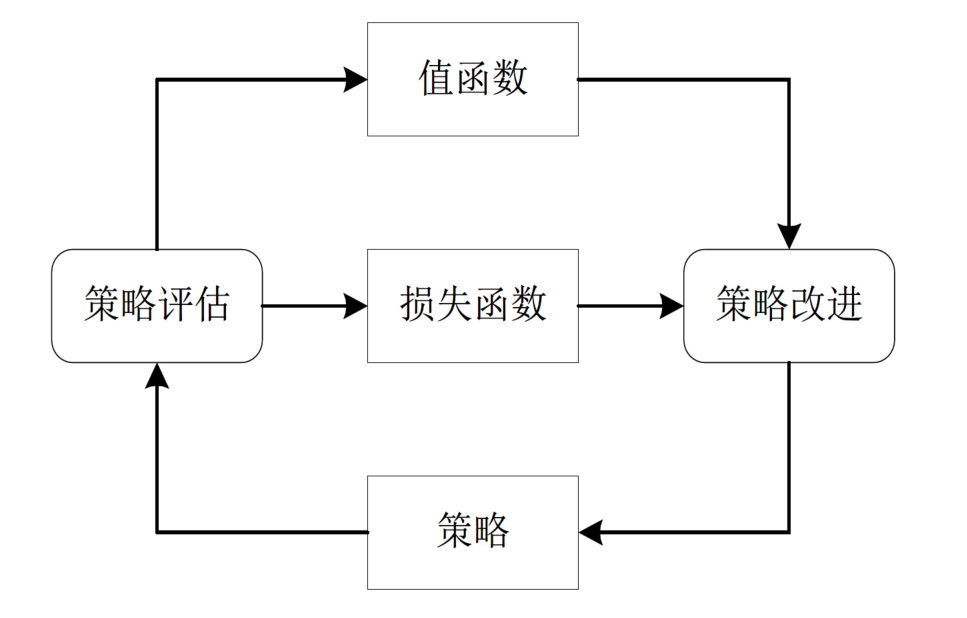
\includegraphics[width=8cm]{./pic/fg5.jpg}
		\caption{基于AC框架的深度策略梯度方法的学习结构}
		\label{fg5}
	\end{figure}

	下面阐述一种重要的基于AC框架的深度策略梯度算法。Lillicrap等人利用DQN扩展Q学习算法的思路对确定性策略梯度(Deterministic Policy Gradient,DPG)方法进行改造,提出了一种基于AC框架的深度确定性策略梯度(Deep Deterministic Policy Gradient,DDPG)算法,该算法可用于解决连续动作空间上的DRL问题。DDPG分别使用参数为$\theta^\mu$和$\theta^Q$的深度神经网络来表示确定性策略$a=\pi(s|\theta^\mu)$和值函数$Q(s,a|\theta^Q)$。其中,策略网络用来更新策略,对应AC框架中的行动者;值网络用来逼近状态动作对的值函数,并提供梯度信息,对应AC框架中的评论家。在DDPG中,目标函数被定义为带折扣的奖赏和:
	\begin{equation}
		\label{eq23}
		J(\theta^\mu)=E_{\theta^\mu}[r_1+\gamma r_2+\gamma^2r_3+\dots]
	\end{equation}
	然后,采用随机梯度下降方法来对目标函数进行端对端的优化。Silver等人证明了目标函数关于$\theta^\mu$的梯度等价于Q值函数关于$\theta^\mu$的期望梯度:
	\begin{equation}
		\label{eq24}
		\frac{\partial J(\theta^\mu)}{\partial \theta^\mu}=E_s[\frac{\partial Q(s,a|\theta^Q)}{\partial \theta^\mu}]
	\end{equation}
	根据确定性策略$a=\pi(s|\theta^\mu)$可得:
	\begin{equation}
		\label{eq25}
		\frac{\partial J(\theta^\mu)}{\partial \theta^\mu}=E_s[\frac{\partial Q(s,a|\theta^Q)}{\partial a}\frac{\partial \pi(s|\theta^\mu)}{\partial \theta^\mu}]
	\end{equation}
	通过DQN中更新值网络的方法来更新评论家网络,此时的梯度信息为:
	\begin{equation}
		\label{eq26}
		\frac{\partial J(\theta^Q)}{\partial \theta^Q}=E_{s,a,r,s'\sim D}[(y-Q(s,a|\theta^Q))\frac{\partial Q(s,a|\theta^Q)}{\partial \theta^Q}]
	\end{equation}
	其中,$y=r+\gamma Q(s',\pi(s'|\hat{\theta ^\mu})|\hat{\theta ^Q})$,$\hat{\theta ^\mu}$和$\hat{\theta ^Q}$分别表示目标策略网络和目标值网络的参数。DDPG使用经验回放机制从D中获得训练样本,并将由Q值函数关于动作的梯度信息从评论家网络传递给行动者网络。并根据式\ref{eq25}沿着提升Q的方向更新策略网络的参数。
	
	实验表明,DDPG不仅在一系列连续动作空间的任务中表现稳定,而且求得最优解所需要的时间步也远远少于DQN。与基于值函数的DRL方法相比,基于AC框架的深度策略梯度方法优化策略效率更高、求解速度更快。
	
	然而在有噪声干扰的复杂环境下,策略一般都具有一定的随机性。DDPG使用确定性的策略梯度方法。对于随机环境的场景,该方法并不适用。针对此问题,Heess等人提出了一种适用于连续动作空间任务的通用框架,称为随机值梯度(Stochastic Value Gradient,SVG)方法。SVG使用“再参数化”(re-parameterization)的数学技巧来学习环境动态性的生成模型,将确定性策略梯度方法扩展为一种随机环境下的策略优化过程。Balduzzi等人基于相容的值函数逼近器(compatible function approximation)理论,提出了值梯度反向更新(Value-Gradient Backpropagation,GProp)方法。Peng等人融合多个策略网络和对应的值网络,提出了一种基于混合型行动者评论家指导(Mixture of Actor Critic Experts,MACE)的深度策略梯度方法。该方法在自适应机器人控制任务中取得了实质性的进展。MACE相比于单个AC框架指导的深度策略梯度方法,有着更快的学习速度。随后,Heess等人使用循环神经网络,进一步扩展了DPG和SVG算法的适用范围,提出了循环确定性策略梯度(Recurrent Deterministic Policy Gradient,RDPG)和循环随机值梯度(Recurrent Stochastic Value Gradient,RSVG)方法。RDPG和RSVG可以处理一系列部分可观察场景下连续动作的控制任务。Hausknecht等人进一步将深度策略梯度方法扩展到了参数化的连续动作空间问题中。此后,Schulman等人提出了一种形式化的随机计算图模型(stochastic computation graphs),开展了同时包含随机性和确定性操作的复杂深度策略梯度的研究。
	
	\subsection{异步优势行动者评论家算法}
	不同类型的深度神经网络为DRL中策略优化任务提供了高效运行的表征形式。为了缓解传统策略梯度方法与神经网络结合时出现的不稳定性,各类深度策略梯度方法(如DDPG、SVG等)都采用了经验回放机制来消除训练数据间的相关性。然而经验回放机制存在两个不足之处:
	\begin{enumerate}
		\item agent与环境的每次实时交互都需要耗费很多的内存和计算力;
		\item 经验回放机制要求agent采用离策略(off-policy)方法来进行学习,而离策略方法只能基于旧策略生成的数据进行更新。
	\end{enumerate}
	针对这些问题,Mnih等人根据异步强化学习(Asynchronous Reinforcement Learning,ARL)的思想,提出了一种轻量级的DRL框架,该框架可以使用异步的梯度下降法来优化网络控制器的参数,并可以结合多种RL算法。其中,异步的优势行动者评论家算法(Asynchronous Advantage Actor-Critic,A3C)在各类连续动作空间的控制任务上表现的最好。
	
	具体地,A3C算法利用CPU多线程的功能并行、异步地执行多个agent。因此在任意时刻,并行的agent都将会经历许多不同的状态,去除了训练过程中产生的状态转移样本之间的关联性。因此这种低消耗的异步执行方式可以很好地替代经验回放机制。
	
	A3C算法在训练时降低了对硬件的要求。深度策略梯度算法十分依赖计算能力很强的图形处理器(Graphics Processing Unit,GPU),而A3C算法在实际的操作过程中只需要一个标准的多核CPU。由表\ref{tb1}可知,A3C算法通过应用多线程技术,降低了模型对硬件的需求,在训练时间更少的情况下,A3C算法在Atari 2600游戏任务上的平均性能有明显提升。而且A3C算法能够只根据原始的视觉输入学习到行走3D迷宫的有效策略。此外,A3C算法还可以广泛应用于各种连续动作空间问题。综上所述,A3C算法能够广泛应用于各种2D、3D离散和连续动作空间的任务,并且在这些任务中都取得了最佳的效果。这说明A3C是目前最通用和最成功的一种DRL算法。当然,将A3C与近期的一些深度策略梯度算法相结合可能会进一步提升其性能。
	
	\begin{table}[h]
		\caption{不同的DRL模型在57个Atari游戏上的平均耗时以及游戏性能的提升}
		\label{tb1}
		\begin{tabular}{|c|c|c|c|}
			\hline
			模型 & 训练条件 & 训练时间/天 & 平均性能提升 \\
			\hline
			DQN & GPU & 8 & 121.9\% \\
			\hline
			DDQN & GPU & 8 & 332.9\% \\
			\hline
			Dueling DDQN & GPU & 8 & 343.8\% \\
			\hline
			Prioritized DQN & GPU & 8 & 463.6\% \\
			\hline
			A3C,FF & CPU & 1 & 344.1\% \\
			\hline
			A3C,FF & CPU & 4 & 496.8\% \\
			\hline
			A3C,LSTM & CPU & 4 & 623.0\% \\
			\hline
		\end{tabular}
	\end{table}
	除了基于值函数的DRL和基于策略梯度的DRL之外,还可以通过增加额外的人工监督来促进策略搜索的过程,即为基于搜索与监督的DRL的核心思想。蒙特卡洛树搜索(Monte Carlo Tree Search,MCTS)作为一种经典的启发式策略搜索方法,被广泛用于游戏博弈问题中的行动规划。因此在基于搜索与监督的DRL方法中,策略搜索一般是通过MCTS来完成的。例如Google公司的AlphaGo围棋算法就将深度神经网络和MCTS相结合,并取得了卓越的成就。
	
	
	\chapter{全文总结与展望}
	
	\section{全文总结}
	本文以时域积分方程方法为研究背景,主要对求解时域积分方程的时间步进算法以及两层平面波快速算法进行了研究。
	
	\section{后续工作展望}
	时域积分方程方法的研究近几年发展迅速,在本文研究工作的基础上,仍有以下方向值得进一步研究:
	
	\thesisacknowledgement
	在攻读博士学位期间,首先衷心感谢我的导师XXX教授
	
	
	\thesisloadbibliography[nocite]{reference}
	
	%
	% Uncomment following codes to load bibliography database with native
	% \bibliography command.
	%
	% \nocite{*}
	% \bibliographystyle{thesis-uestc}
	% \bibliography{reference}
	%
	
	\thesisappendix
	
	\thesisloadachievement{publications}
	
	
	\thesistranslationoriginal
	\section{A Tight Upper Bound on Bit Error Rate}
	
	
	\thesistranslationchinese
	
	\section{基于多载波索引键控的正交频分多路复用系统模型}
	
\end{document}
